\chapter{Additional Design Diagrams and Wireframes}
\label{app:diagrams_catalog}

\section{System Interface Wireframes}
The user interface follows the Human-Computer Interaction (HCI) design system developed for Digital Mohalla, accommodating varying technical literacies within local communities.

\begin{figure}[htbp]
\centering
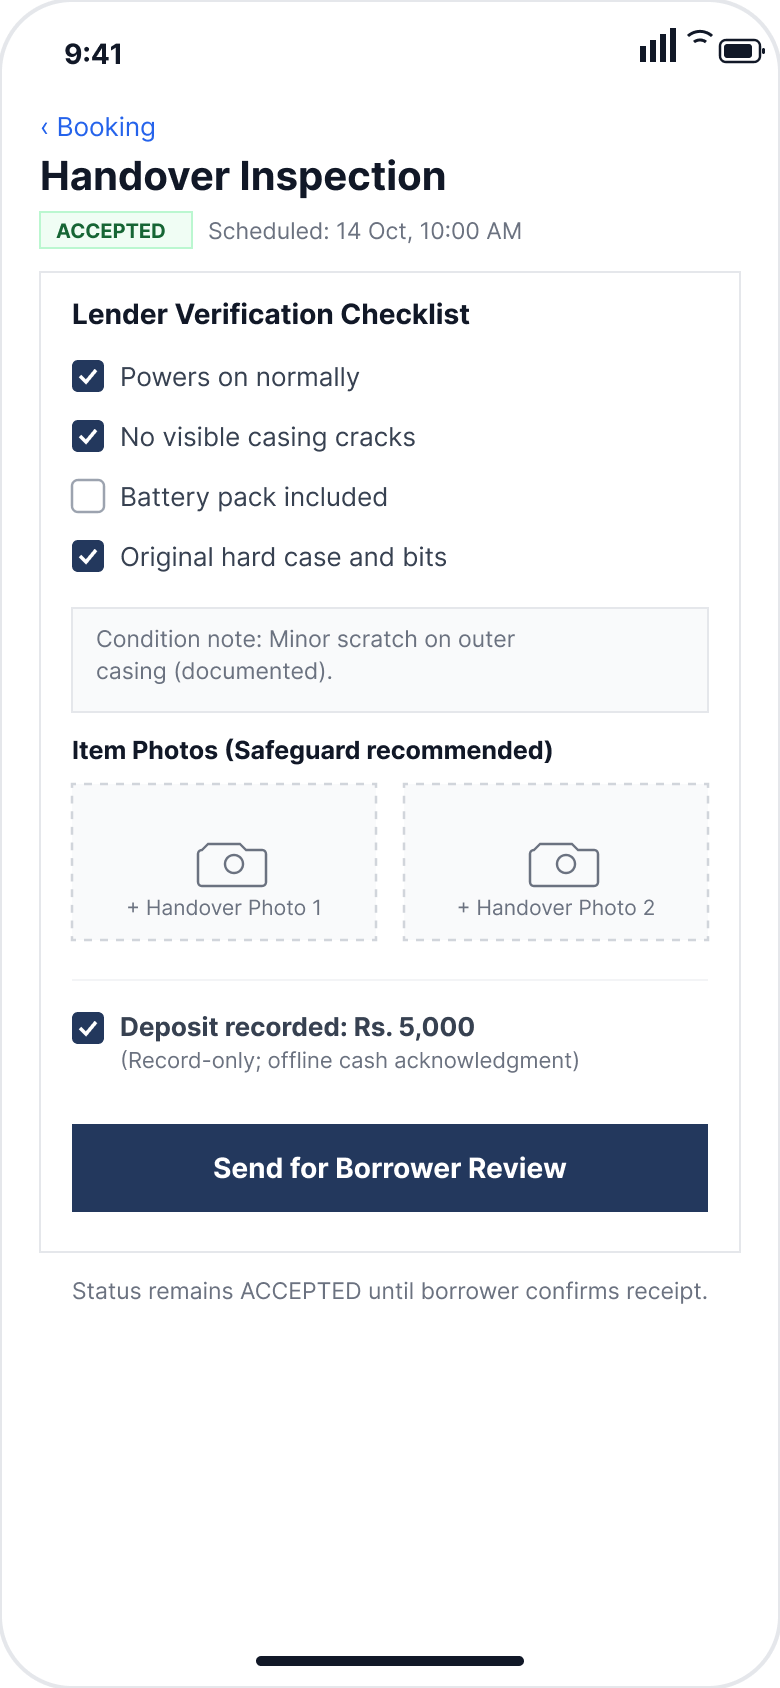
\includegraphics[width=0.45\textwidth]{figures/W3a_Handover_Inspection_Lender_1.png}
\hfill
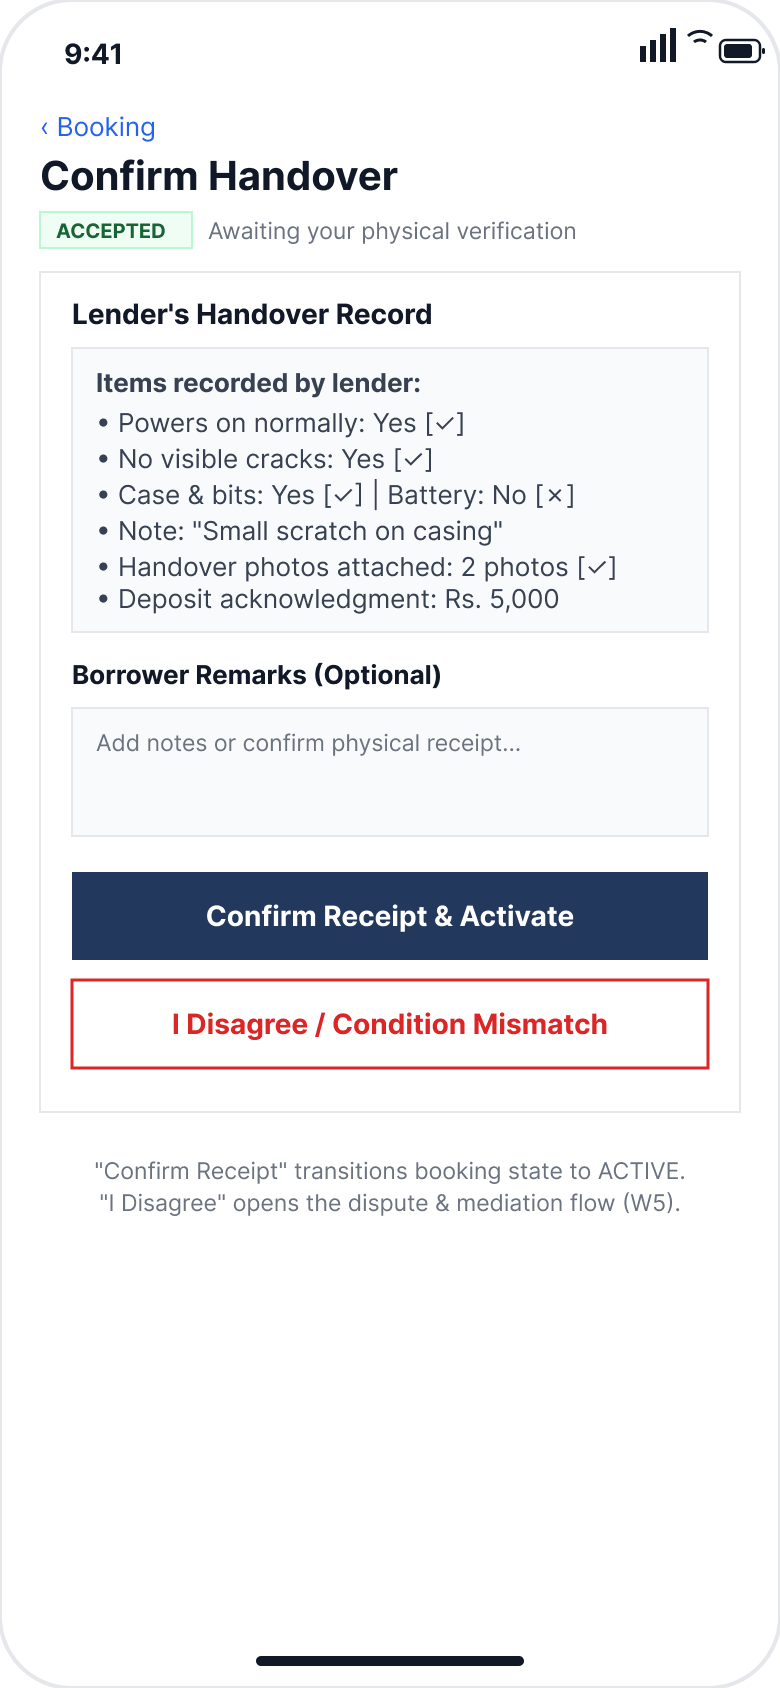
\includegraphics[width=0.45\textwidth]{figures/W3b_Handover_Confirmation_Borrower_1.png}
\caption{Handover Inspection Screens: (Left) Lender Inspection Checklist (W3a); (Right) Borrower Confirmation (W3b)}
\label{fig:wireframes_handover}
\end{figure}

\begin{figure}[htbp]
\centering
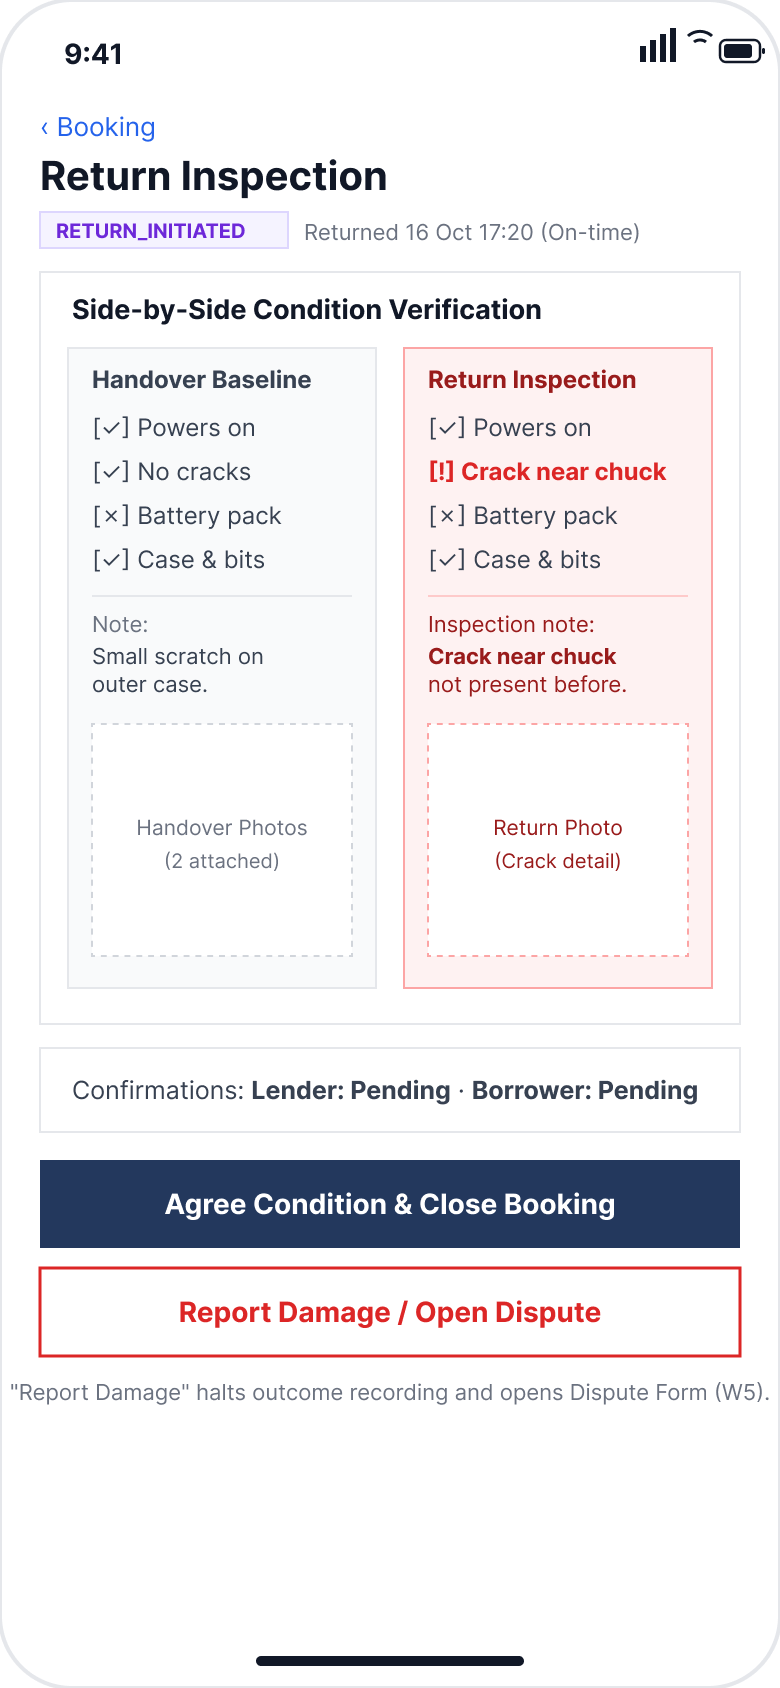
\includegraphics[width=0.45\textwidth]{figures/W4_Return_Inspection_Comparison_1.png}
\hfill
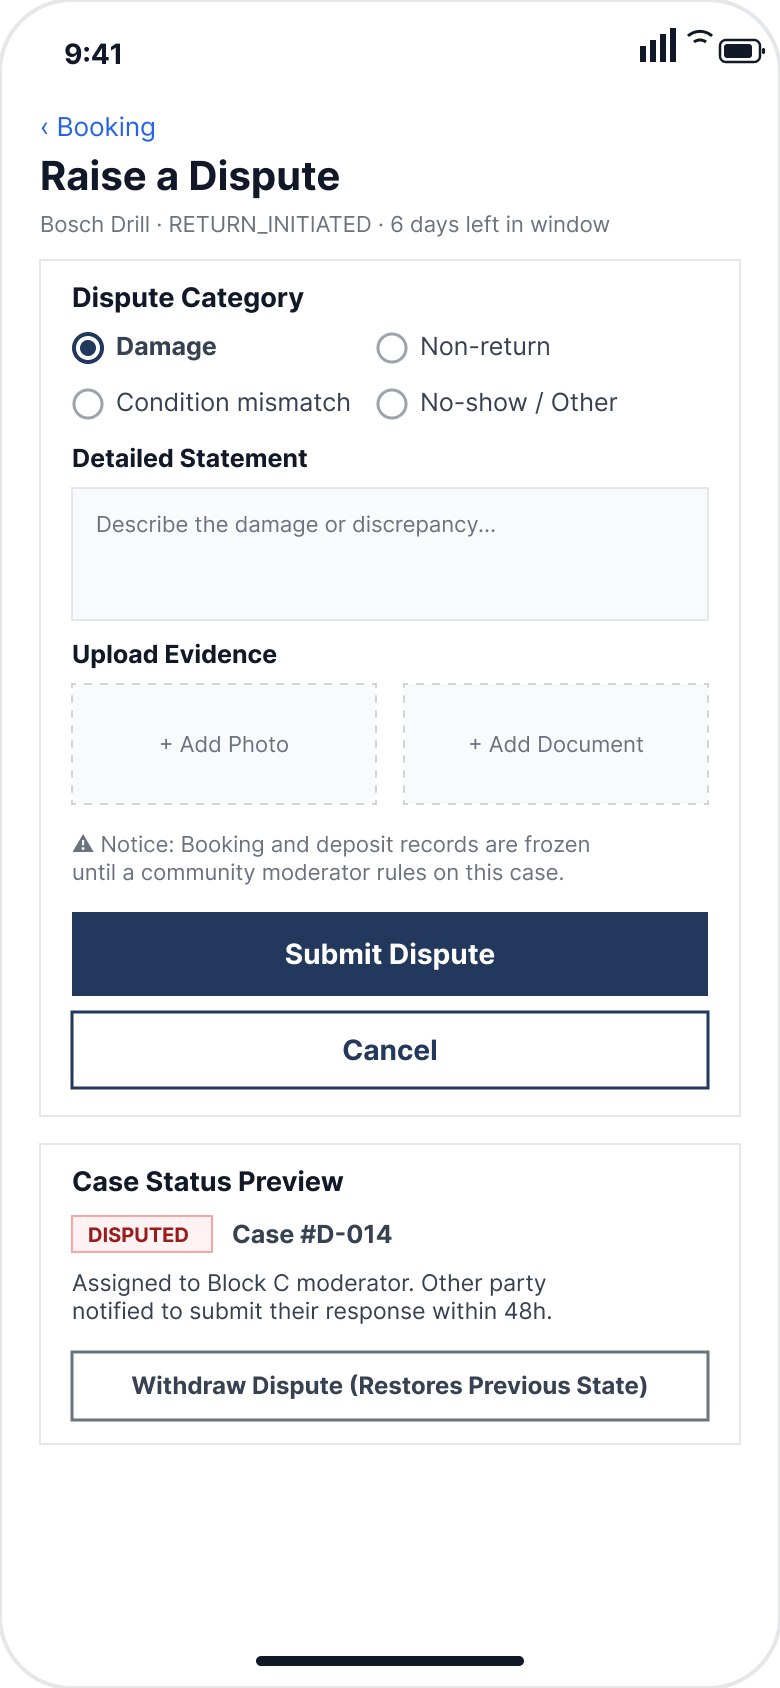
\includegraphics[width=0.45\textwidth]{figures/W5_Dispute_Form_Progress_1.png}
\caption{Return and Dispute Flow: (Left) Return Photographic Comparison (W4); (Right) Dispute Form Submission (W5)}
\label{fig:wireframes_return_dispute}
\end{figure}

\begin{figure}[htbp]
\centering
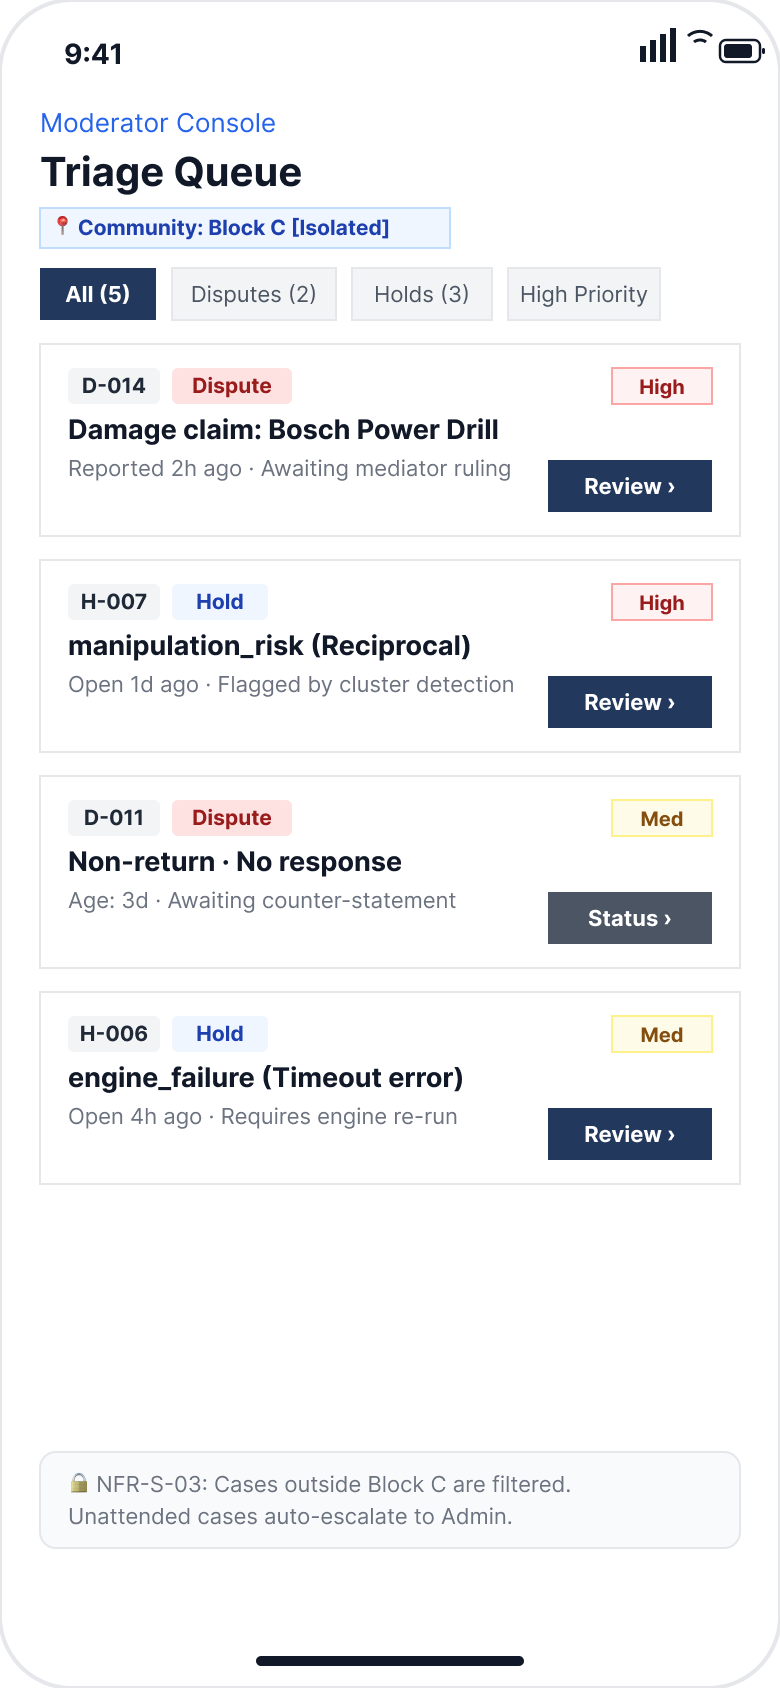
\includegraphics[width=0.45\textwidth]{figures/W6_Moderator_Queue_Mobile_1.png}
\hfill
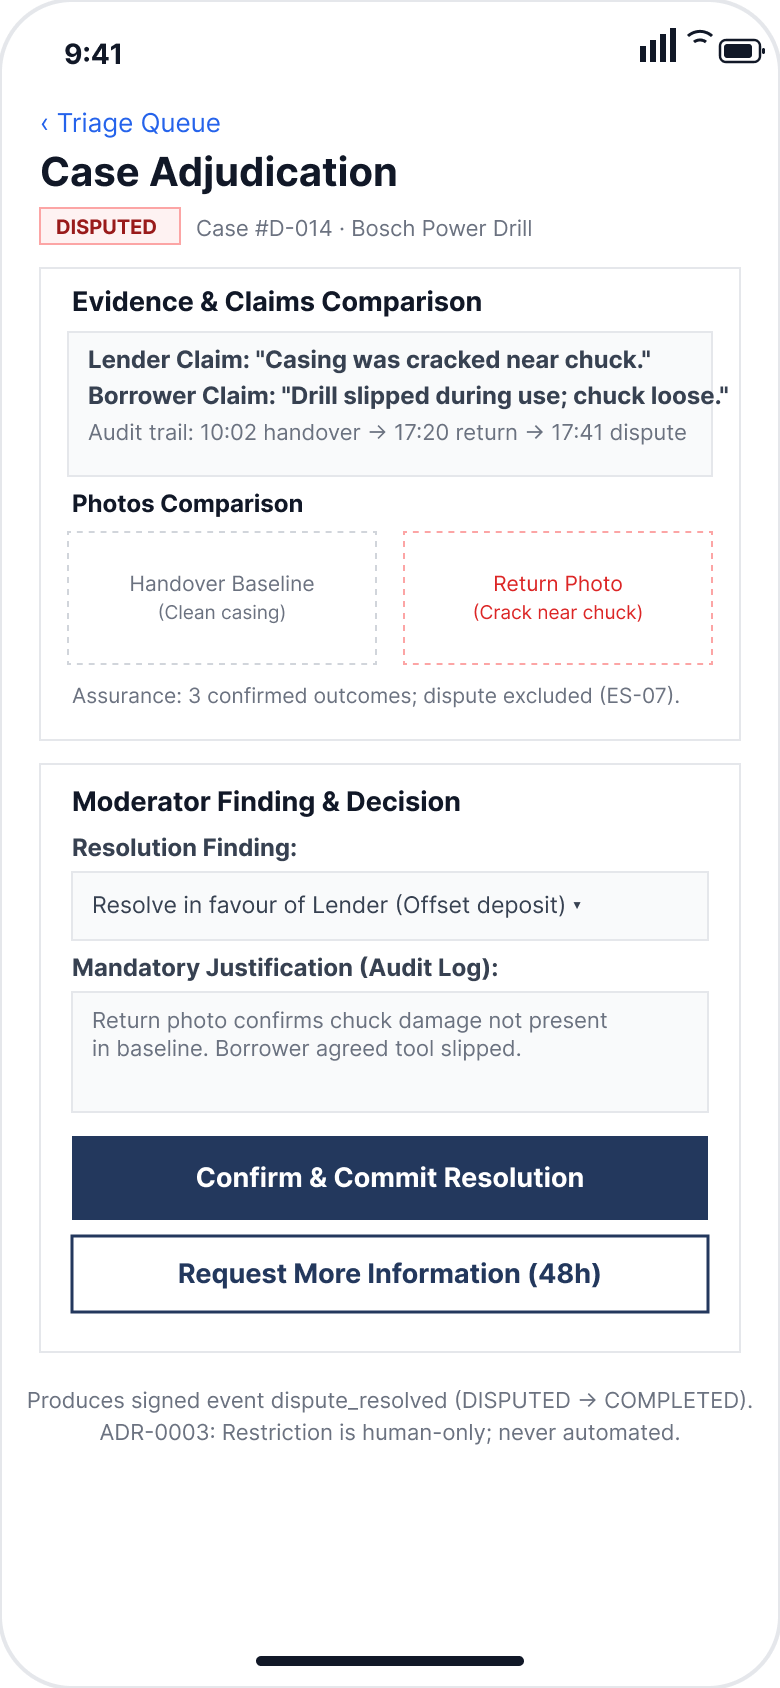
\includegraphics[width=0.45\textwidth]{figures/W7_Moderator_Case_Adjudication_Mobile_1.png}
\caption{Moderator Adjudication Interface: (Left) Moderator Escalation Queue (W6); (Right) Case Adjudication and Ruling Screen (W7)}
\label{fig:wireframes_moderator}
\end{figure}

\section{Detailed Domain Class Diagrams}
The domain object model is subdivided across three vertical slices:
\begin{itemize}
    \item \textbf{Slice 1 (Borrowing \& Event Sourcing):} Represents \texttt{BorrowingRequest}, immutable \texttt{LifecycleEvent}, audit logs, and status transitions.
    \item \textbf{Slice 2 (Locality, User Trust, and Social Graph):} Encapsulates coarse locality boundaries, directed trust edges, Bayesian parameters, and indirect path traversal.
    \item \textbf{Slice 3 (Escalation, Disputes, and Moderator Resolution):} Models dispute claims, photographic evidence bundles, and moderator adjudication outcomes.
\end{itemize}

\begin{figure}[htbp]
\centering
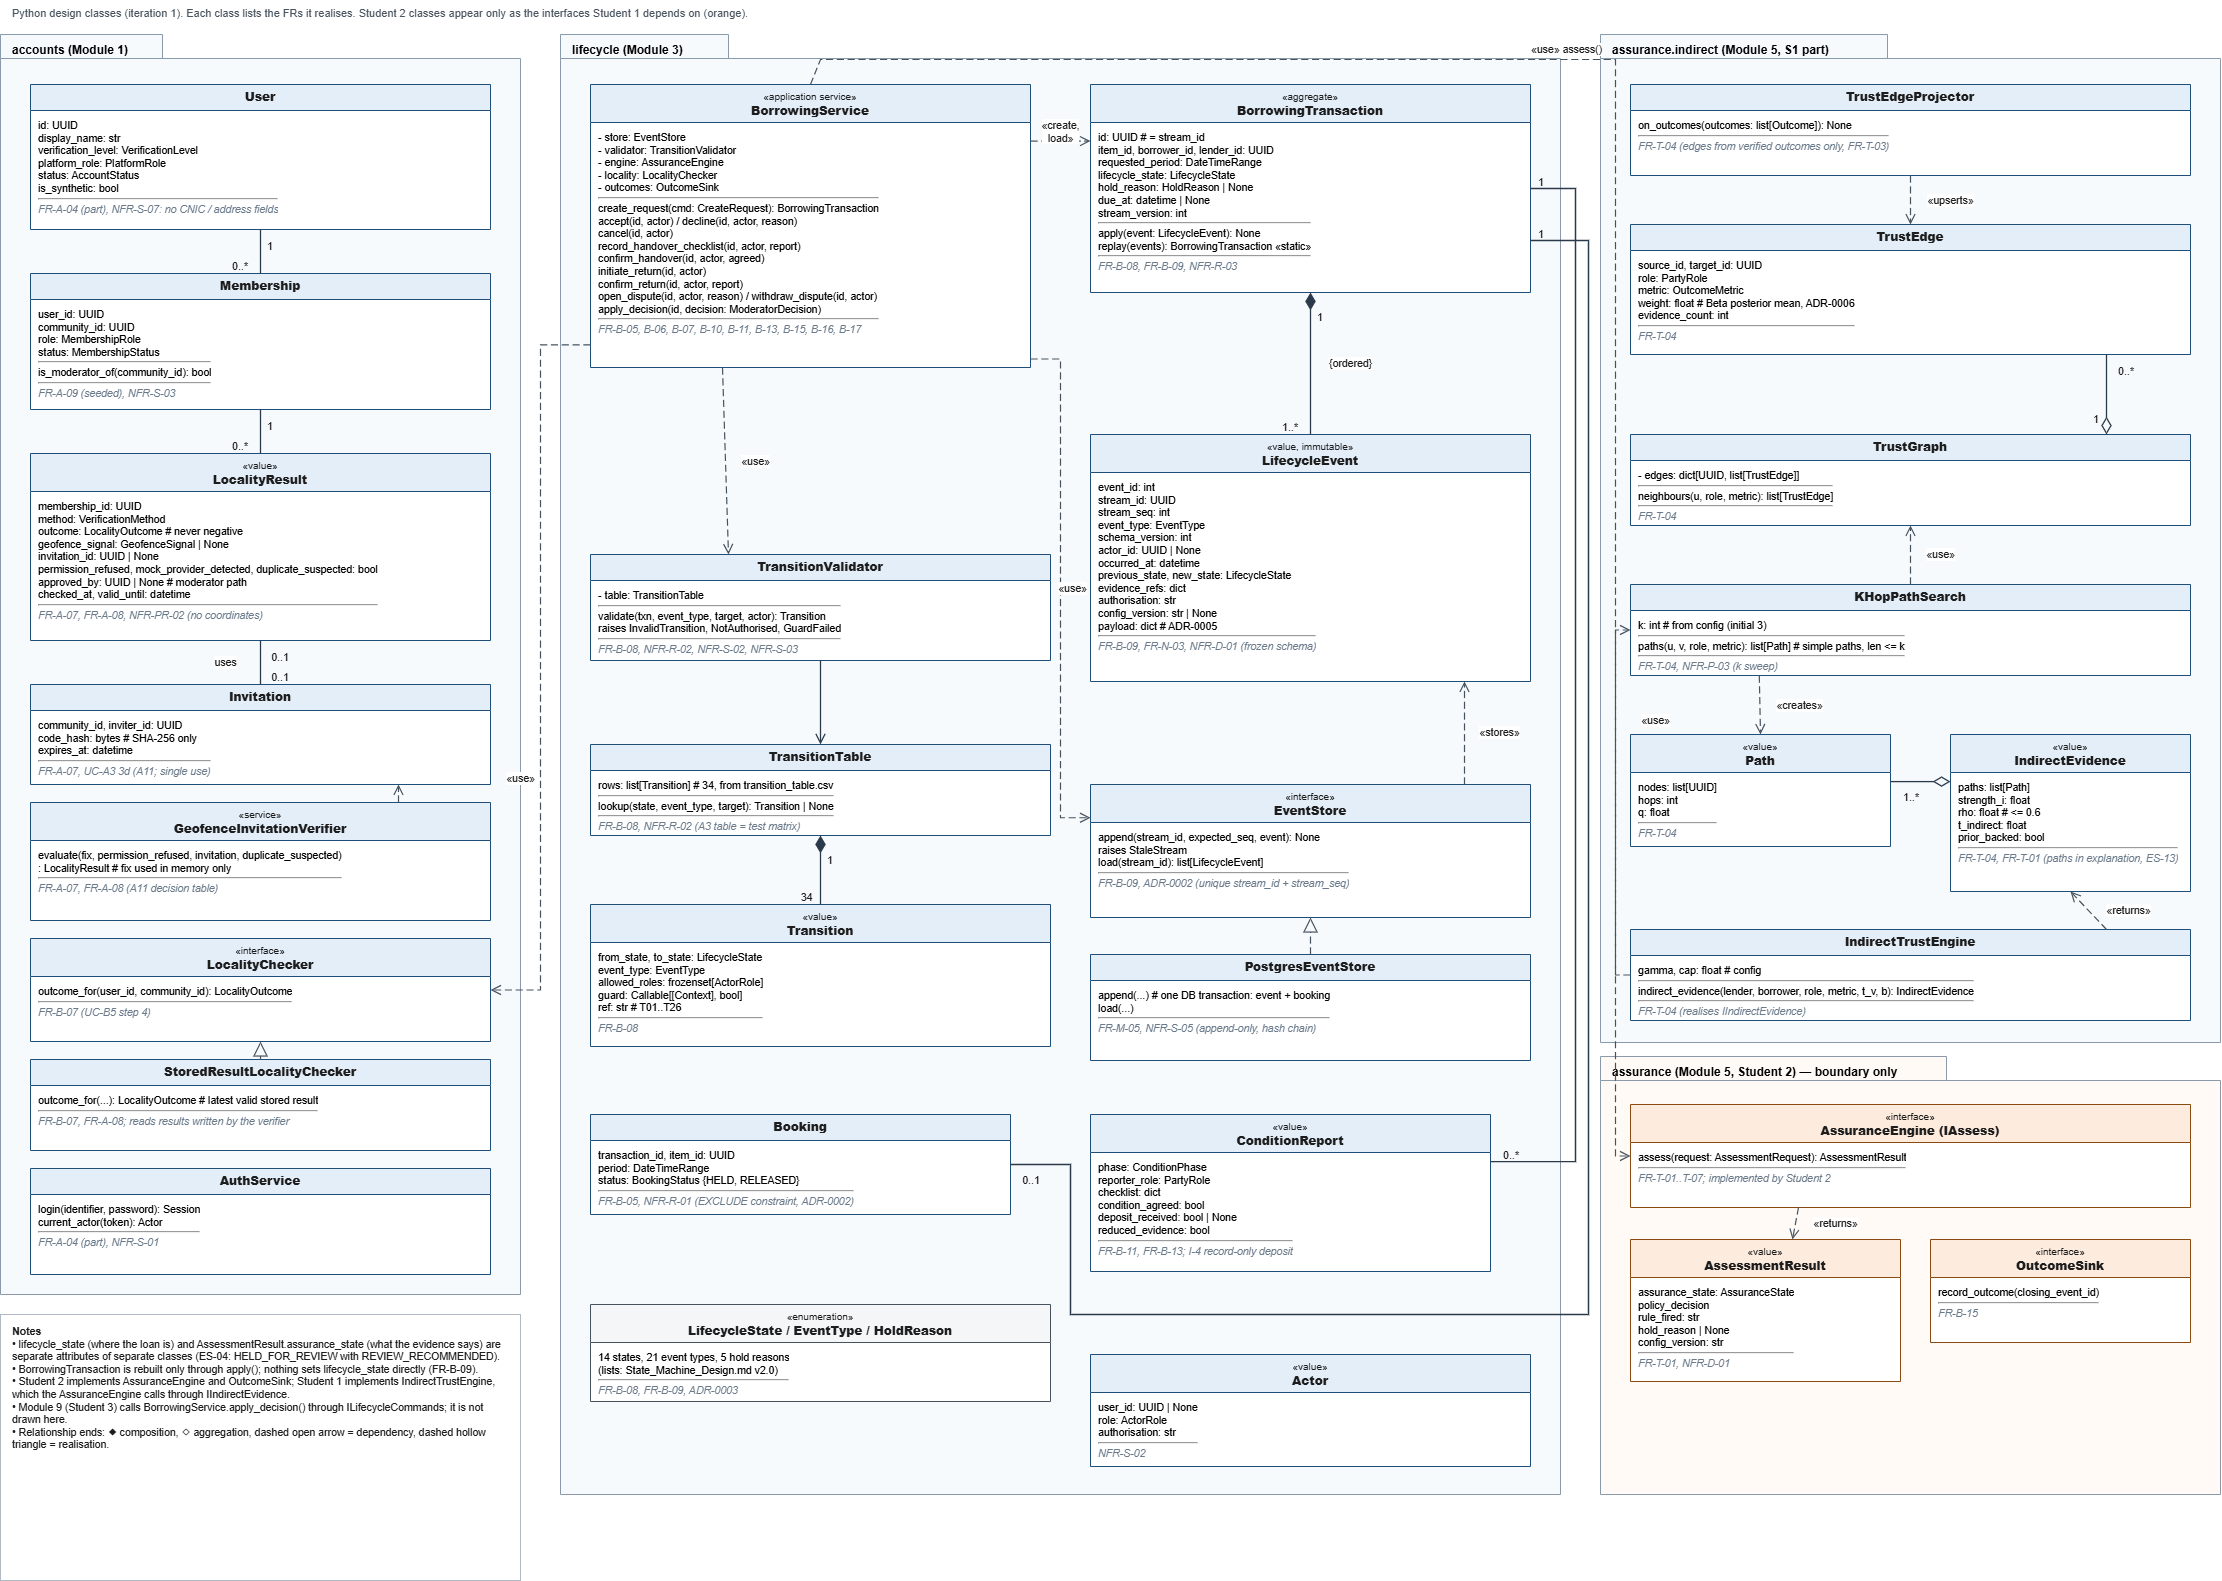
\includegraphics[width=0.85\textwidth]{../../design/05_class_model/class_diagram_s1.drawio.png}
\caption{Domain Class Diagram: Slice 1 (Borrowing and Event Sourcing Core)}
\label{fig:class_s1}
\end{figure}

\begin{figure}[htbp]
\centering
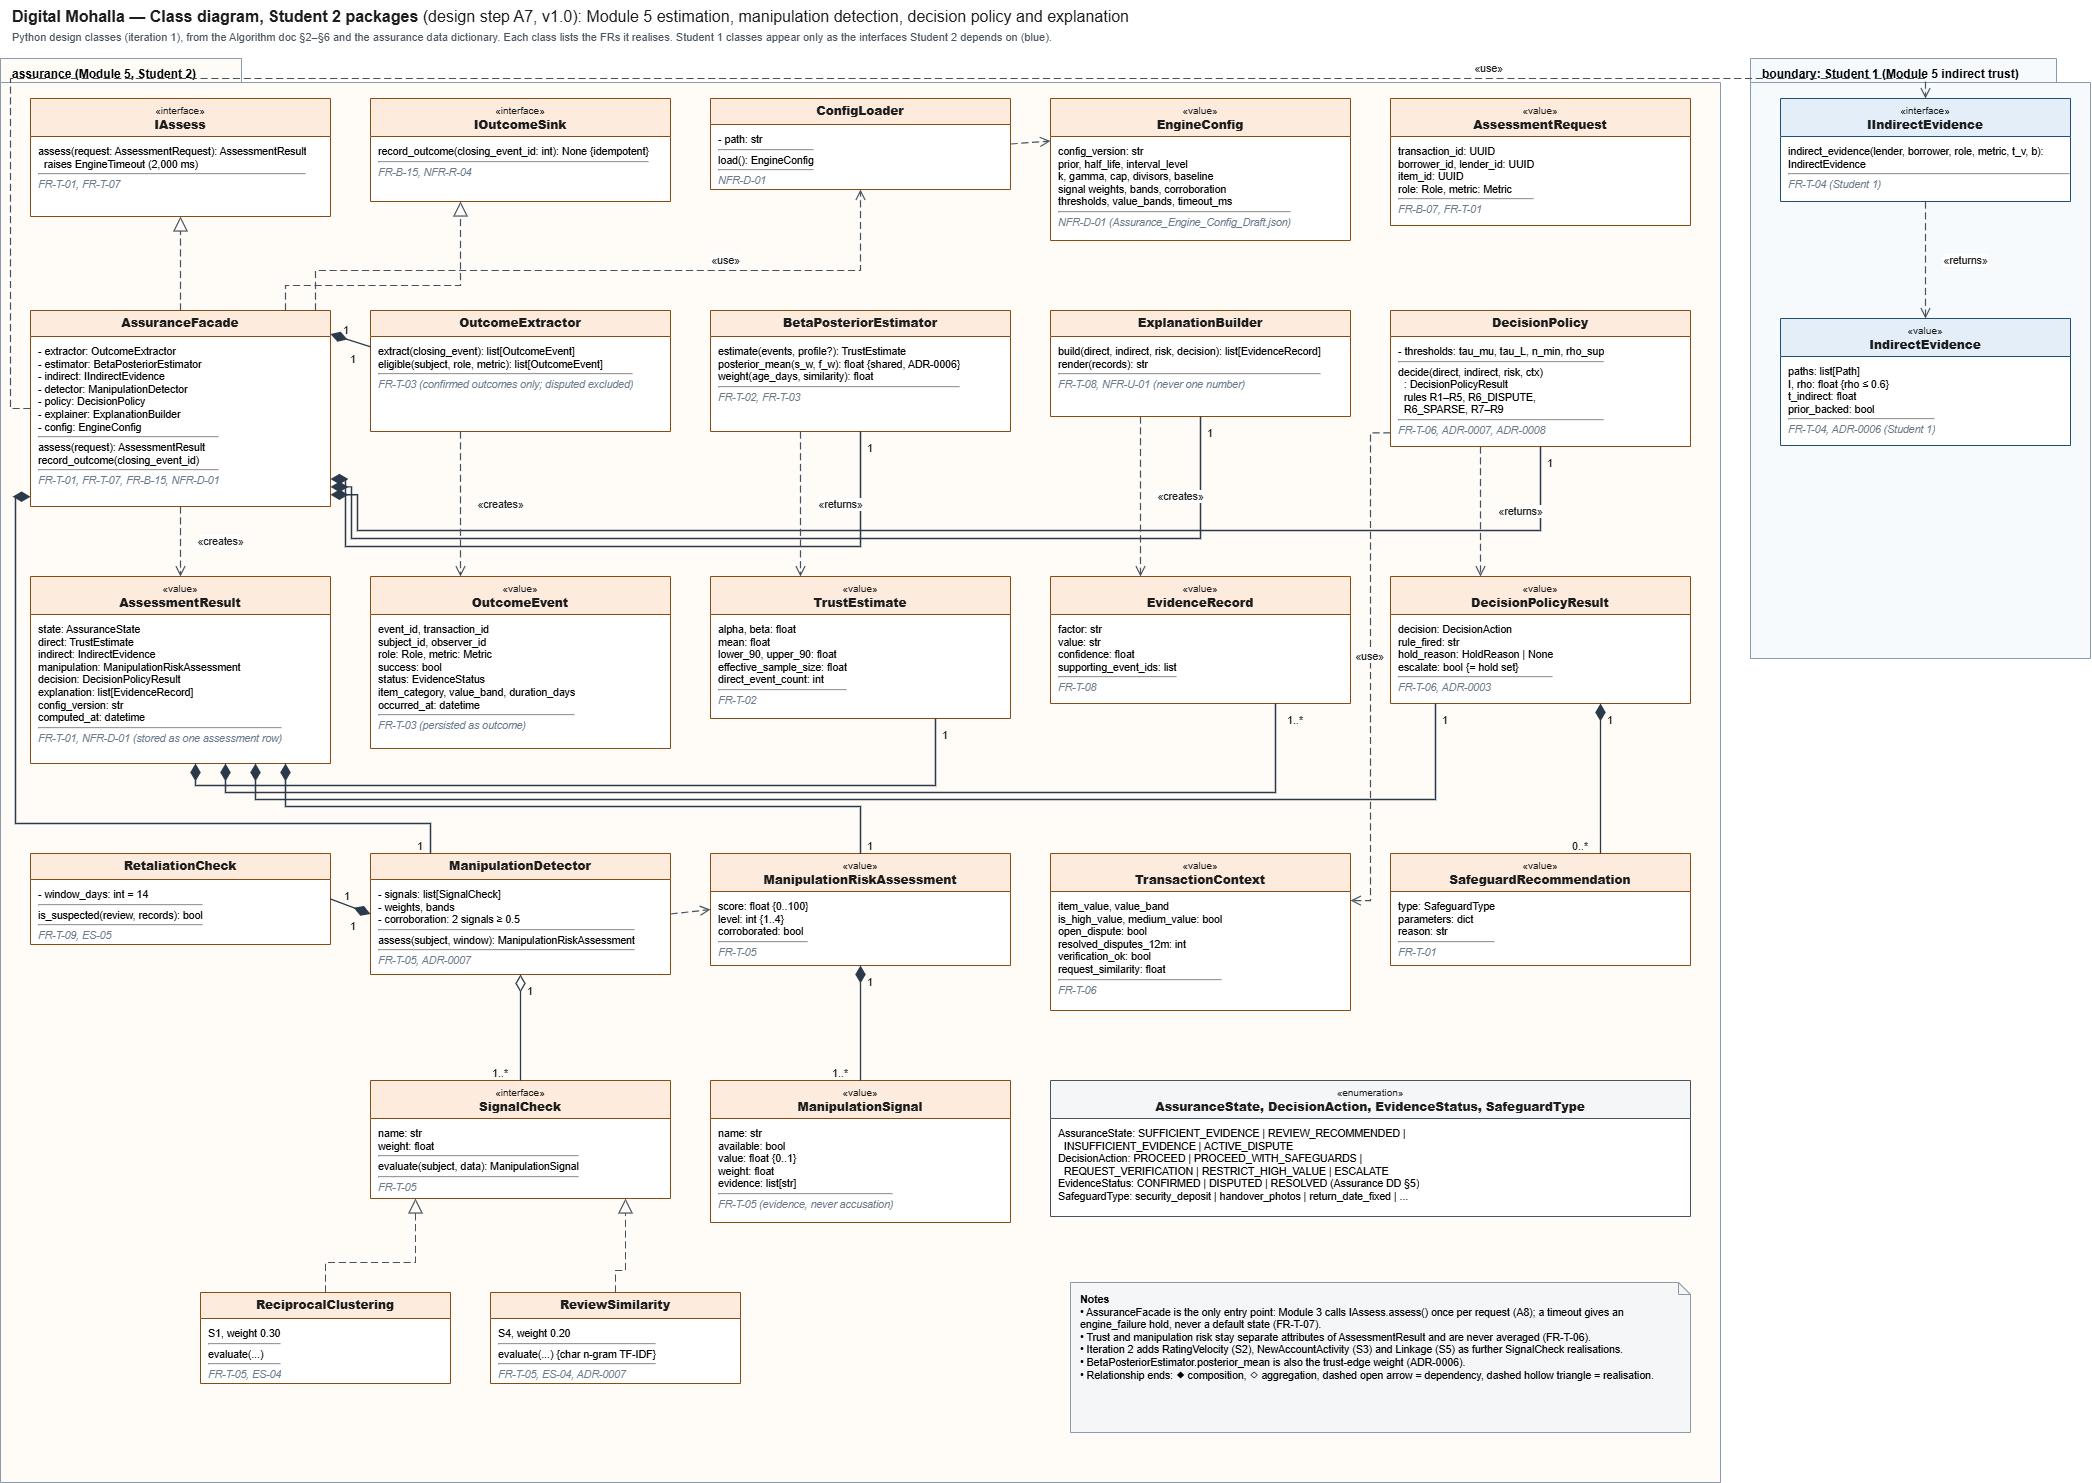
\includegraphics[width=0.85\textwidth]{../../design/05_class_model/class_diagram_s2.drawio.png}
\caption{Domain Class Diagram: Slice 2 (Trust Engine and Locality Graph)}
\label{fig:class_s2}
\end{figure}

\begin{figure}[htbp]
\centering
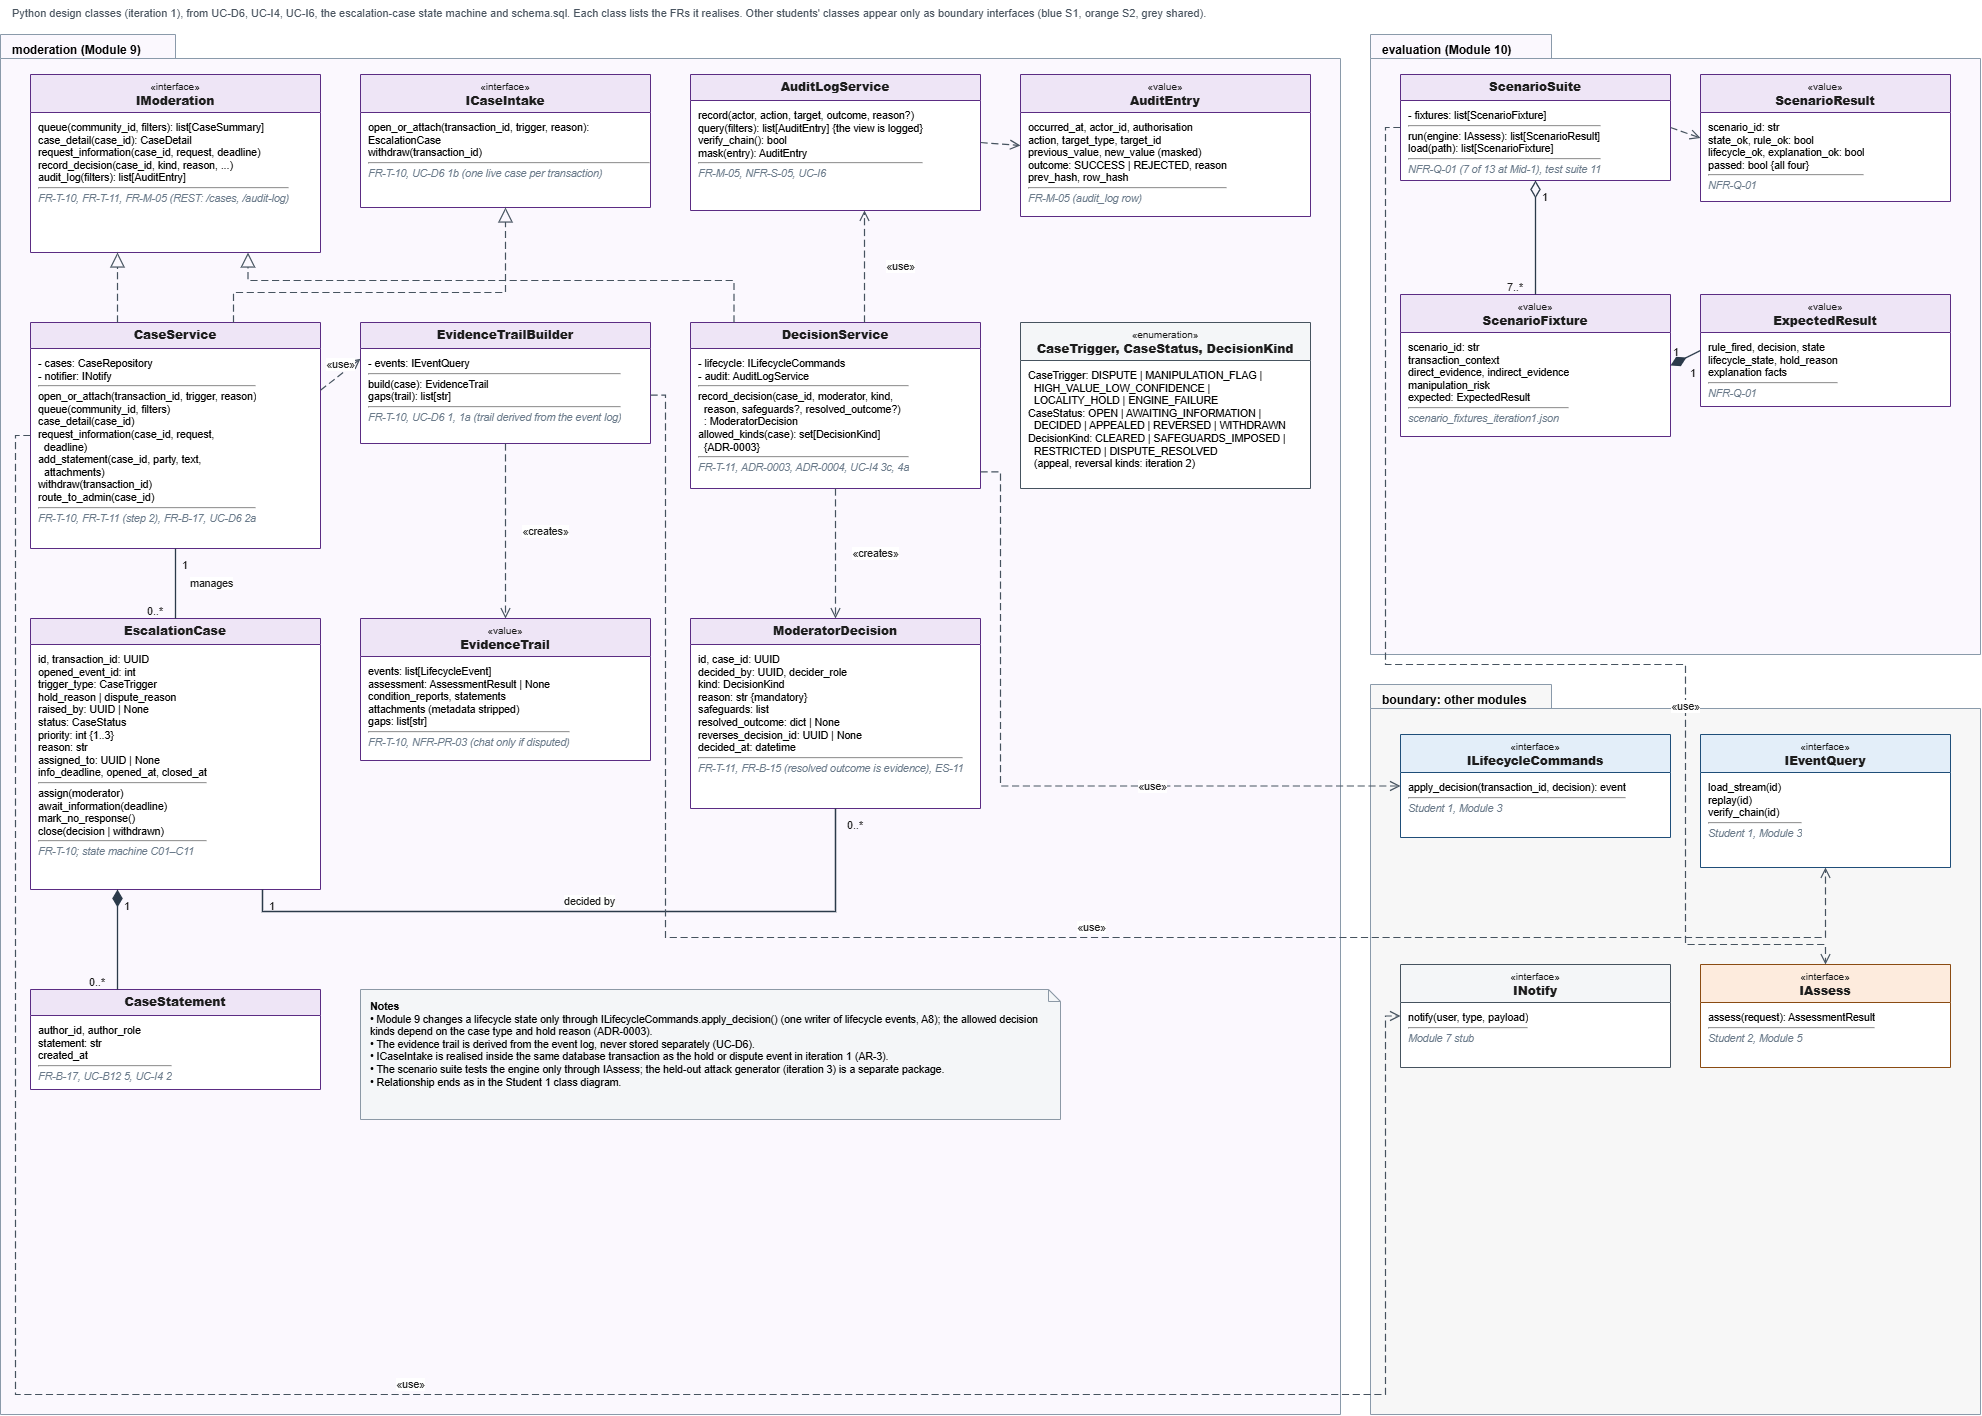
\includegraphics[width=0.85\textwidth]{../../design/05_class_model/class_diagram_s3.drawio.png}
\caption{Domain Class Diagram: Slice 3 (Disputes, Evidence, and Governance)}
\label{fig:class_s3}
\end{figure}

\section{Escalation Case State Machine}
\begin{figure}[htbp]
\centering
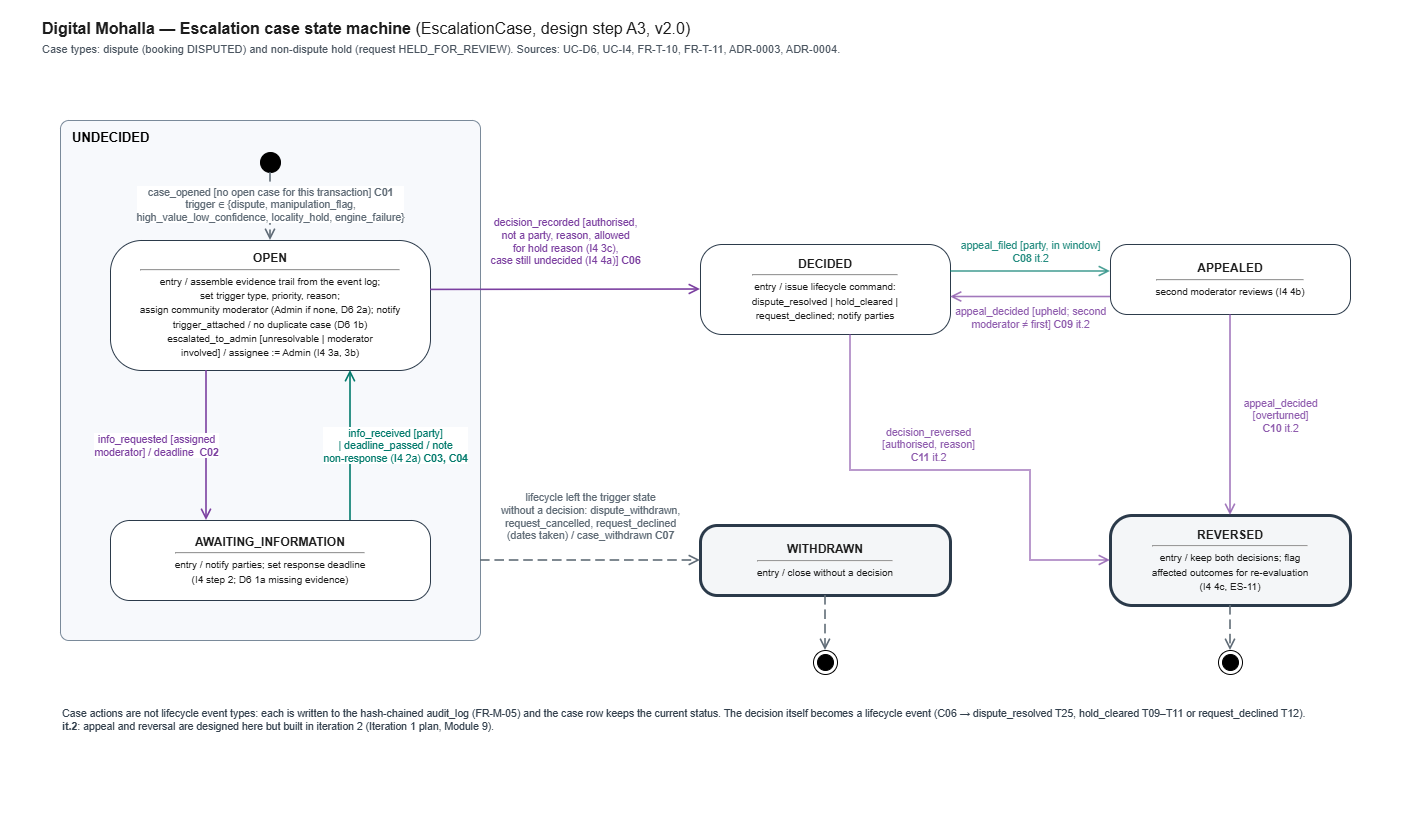
\includegraphics[width=0.85\textwidth]{../../design/07_state_machines/escalation_case_state_machine.drawio.png}
\caption{Escalation Case Lifecycle and Moderator Adjudication State Flow}
\label{fig:escalation_state_machine}
\end{figure}
